\documentclass[10pt,xcolor=pdflatex]{beamer}
\usepackage{newcent}
\usepackage[utf8]{inputenc}
%\usepackage[czech]{babel}
\usepackage{hyperref}
\usepackage{fancyvrb}
\usetheme{FIT}

%%%%%%%%%%%%%%%%%%%%%%%%%%%%%%%%%%%%%%%%%%%%%%%%%%%%%%%%%%%%%%%%%%
\title[Ztrátová komprese plenoptických fotografií]{Ztrátová komprese\\plenoptických fotografií}

\author[]{Drahomír Dlabaja}

\institute[]{Vedoucí práce: Ing. David Bařina, Ph.D.\\
Brno University of Technology, Faculty of Information Technology\\
Bo\v{z}et\v{e}chova 1/2. 612 66 Brno - Kr\'alovo Pole\\
xdlaba02@stud.fit.vutbr.cz}

\date{\today}
%\date{} % bez data

%%%%%%%%%%%%%%%%%%%%%%%%%%%%%%%%%%%%%%%%%%%%%%%%%%%%%%%%%%%%%%%%%%

\begin{document}

\frame[plain]{\titlepage}

\begin{frame}\frametitle{Úvod do problematiky}
  \begin{columns}
    \column{0.6\linewidth}
      \begin{figure}
        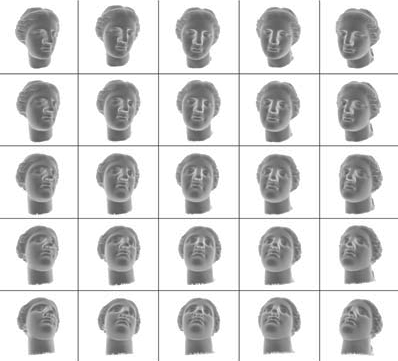
\includegraphics[width=\textwidth]{img/head.png}
      \end{figure}
    \column{0.5\linewidth}
      \centering
      $1400 \times 800 \times 5 \times 5 \times 3 = 84$ MB\\[2em]
      Fotografie je potřeba efektivně komprimovat!
  \end{columns}
\end{frame}

\begin{frame}\frametitle{Existující řešení}
  \begin{columns}
    \column{0.7\linewidth}
    \begin{block}{Jednotlivé pohledy můžeme komprimovat samostatně,}
      \begin{itemize}
        \item JPEG,
        \item JPEG 2000,
        \item H.264,
        \item H.265,
      \end{itemize}
    \end{block}
    \begin{block}{nebo je můžeme vhodně seřadit a komprimovat jako video,}
      \begin{itemize}
        \item H.264,
        \item H.265.
      \end{itemize}
    \end{block}
    \column{0.3\linewidth}
    \begin{figure}
      \includegraphics[width=\textwidth]{img/jpegpleno.pdf}
    \end{figure}
  \end{columns}
\end{frame}

\begin{frame}\frametitle{Moje řešení}
  \begin{center}
    {\Large Plenoptická fotografie jako 4D hyperkvádr}
    \begin{columns}
      \column{0.6\linewidth}
        \begin{itemize}
          \item Dvě dimenze pro index pixelu,
          \item dvě dimenze pro index pohledu,
          \item zrcadlení metody JPEG do čtvrtého rozměru,
          \item bloky $8 \times 8 \times 8 \times 8$ pixelů,
          \item 4D cosinova transformace,
          \item 4D kvantizační tabulka.
        \end{itemize}
      \column{0.5\linewidth}
        \begin{figure}
          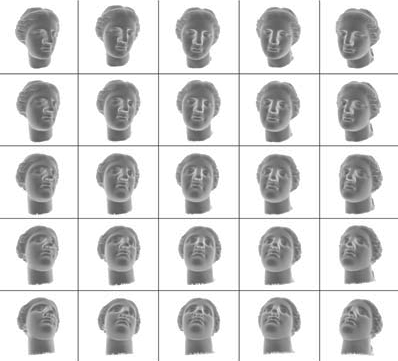
\includegraphics[width=\textwidth]{img/head.png}
        \end{figure}
    \end{columns}
    \vfill
    Využití podobnosti mezi sousedními pohledy.
  \end{center}
\end{frame}

\begin{frame}\frametitle{Přehled práce}
  \begin{itemize}
    \item Implementace metody JPEG pro 2D, 3D a 4D data.
    \item Porovnání efektivity těchto metod.
    \rule{\linewidth}{0.4pt}
    \item Komprese pomocí videokodeků H.264/H.265.
  \end{itemize}
  \begin{figure}
    \includegraphics[width=0.8\textwidth]{img/plot.pdf}
  \end{figure}
\end{frame}


\bluepage{Děkuji za pozornost.}

\end{document}
